
\chapter{Eigenanalysis}
\label{ch:eigen}

The title of this chapter alone is enough to make one's blood run cold. You
might be thinking, ``even if I could pronounce this, would I want to?''

In German, the root \textit{eigen} (pronounced EYE-gun) means something like
``one's own, inherent thing.'' As we'll see, in studying the eigenvectors and
eigenvalues of a matrix -- which is called eigen-analysis -- we're looking at
its deepest, innermost properties. We're peering deep within all the flesh to
see its skeleton. And it turns out this is the key to the most profound
understanding of what a matrix is and does.

\section{Hitting the resonant frequency}

\index{resonant frequency}
\index{frequency, resonant}

We could come at this subject in a bunch of different ways, but let me start
with the first thing that clicked for me. At the time, I was reminded of the
phenomenon of a ``resonant frequency'' that some systems exhibit.

\index{playground}
\index{swing}

You'll remember this effect if you've ever been on a playground swing. When
somebody pushes you (or when you pump your legs to ``push'' yourself) you have
to do it at the right time and at the right pace. The swing has a natural
frequency of oscillation, and it resists being pushed faster or slower than
that. If you find you're swinging from back to front every two seconds, you'll
have to pump your legs every two seconds. Even if you have thighs like Dwayne
Johnson, trying to pump every 1.5 seconds or every second will do you no good.
But timing it so you pump your legs at exactly the string's resonant frequency
will make you go higher and higher.

\index{Tacoma Narrows Bridge}
\index{bridge}
\index{Slinky}

There are other famous examples of the resonant frequency phenomenon. Perhaps
you've heard of the Tacoma Narrows Bridge (if you've never seen it, check out
the video on
\href{https://www.youtube.com/watch?v=j-zczJXSxnw}{\underline{YouTube}}). It
was a beautiful double-lane suspension bridge in Washington State that crossed
the Puget Sound -- at the time, the third-largest suspension bridge in the
world. Incredibly, on November 7th, 1940, it began to wobble with increasing
intensity as crosswinds dangerously amplified its internal structural
vibrations. It looked like a 3,000-foot-long undulating Slinky.\footnote{The
classic ``Slinky'' toy, by the way, is another example of a system that has a
resonant frequency. You can't make it go down the stairs any faster or slower
than it wants to go.} Moments later, the concrete cracked and split and the
entire bridge completely collapsed and fell into the Puget Sound. Luckily,
drivers had wisely stopped crossing it minutes before, and the only actual
casualty was a cocker spaniel.

\begin{center}
\label{tacoma}
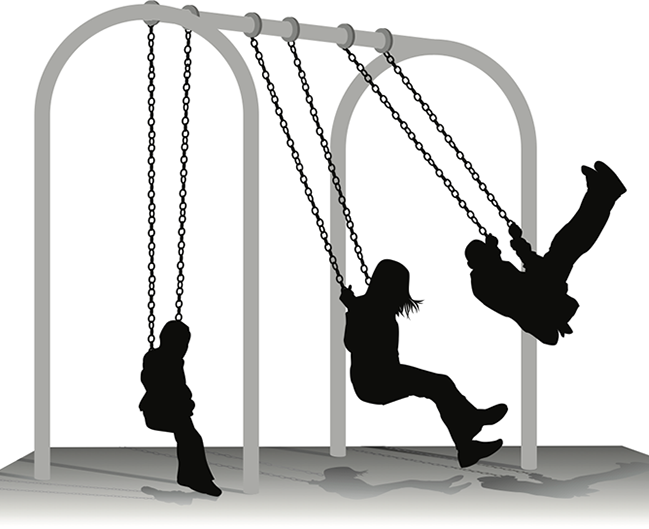
\includegraphics[width=0.45\textwidth]{swing.png}
\quad
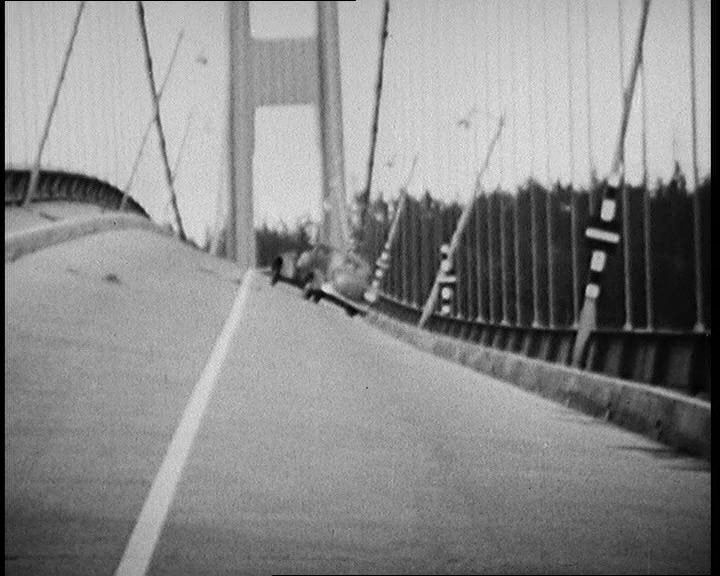
\includegraphics[width=0.45\textwidth]{tacoma.jpg}
\end{center}

The reasons for the Tacoma Bridge catastrophe are a bit complex, but a key
contributing factor was that a very specific rate of oscillation -- a ``sweet
spot,'' though it was hardly sweet for those involved -- caused the
fluctuations to build on each other instead of being dampened. It's like the
Tacoma Bridge \textit{wanted} to vibrate at a certain frequency, just like a
playground swing has an intrinsic rhythm that the child can't speed up or slow
down.

Yet another example: this is basically how every non-percussive musical
instrument works. A piano or guitar string tuned to middle~C has a certain
length and tension, which causes it to resist vibrations at any frequency other
than exactly 262 per second. Thus, when you strike it, only the 262
Hz\footnote{``Hz,'' pronounced ``hertz,'' is a unit meaning ``cycles
(backs-and-forths) per second.'' Every musical note is defined by a particular
frequency. The lowest key on the piano is 27.5 Hz, and the highest is 4,186
Hz.} tone gains any traction, and the instrument sounds a clear, pure note.

\begin{center}
\label{slinky}
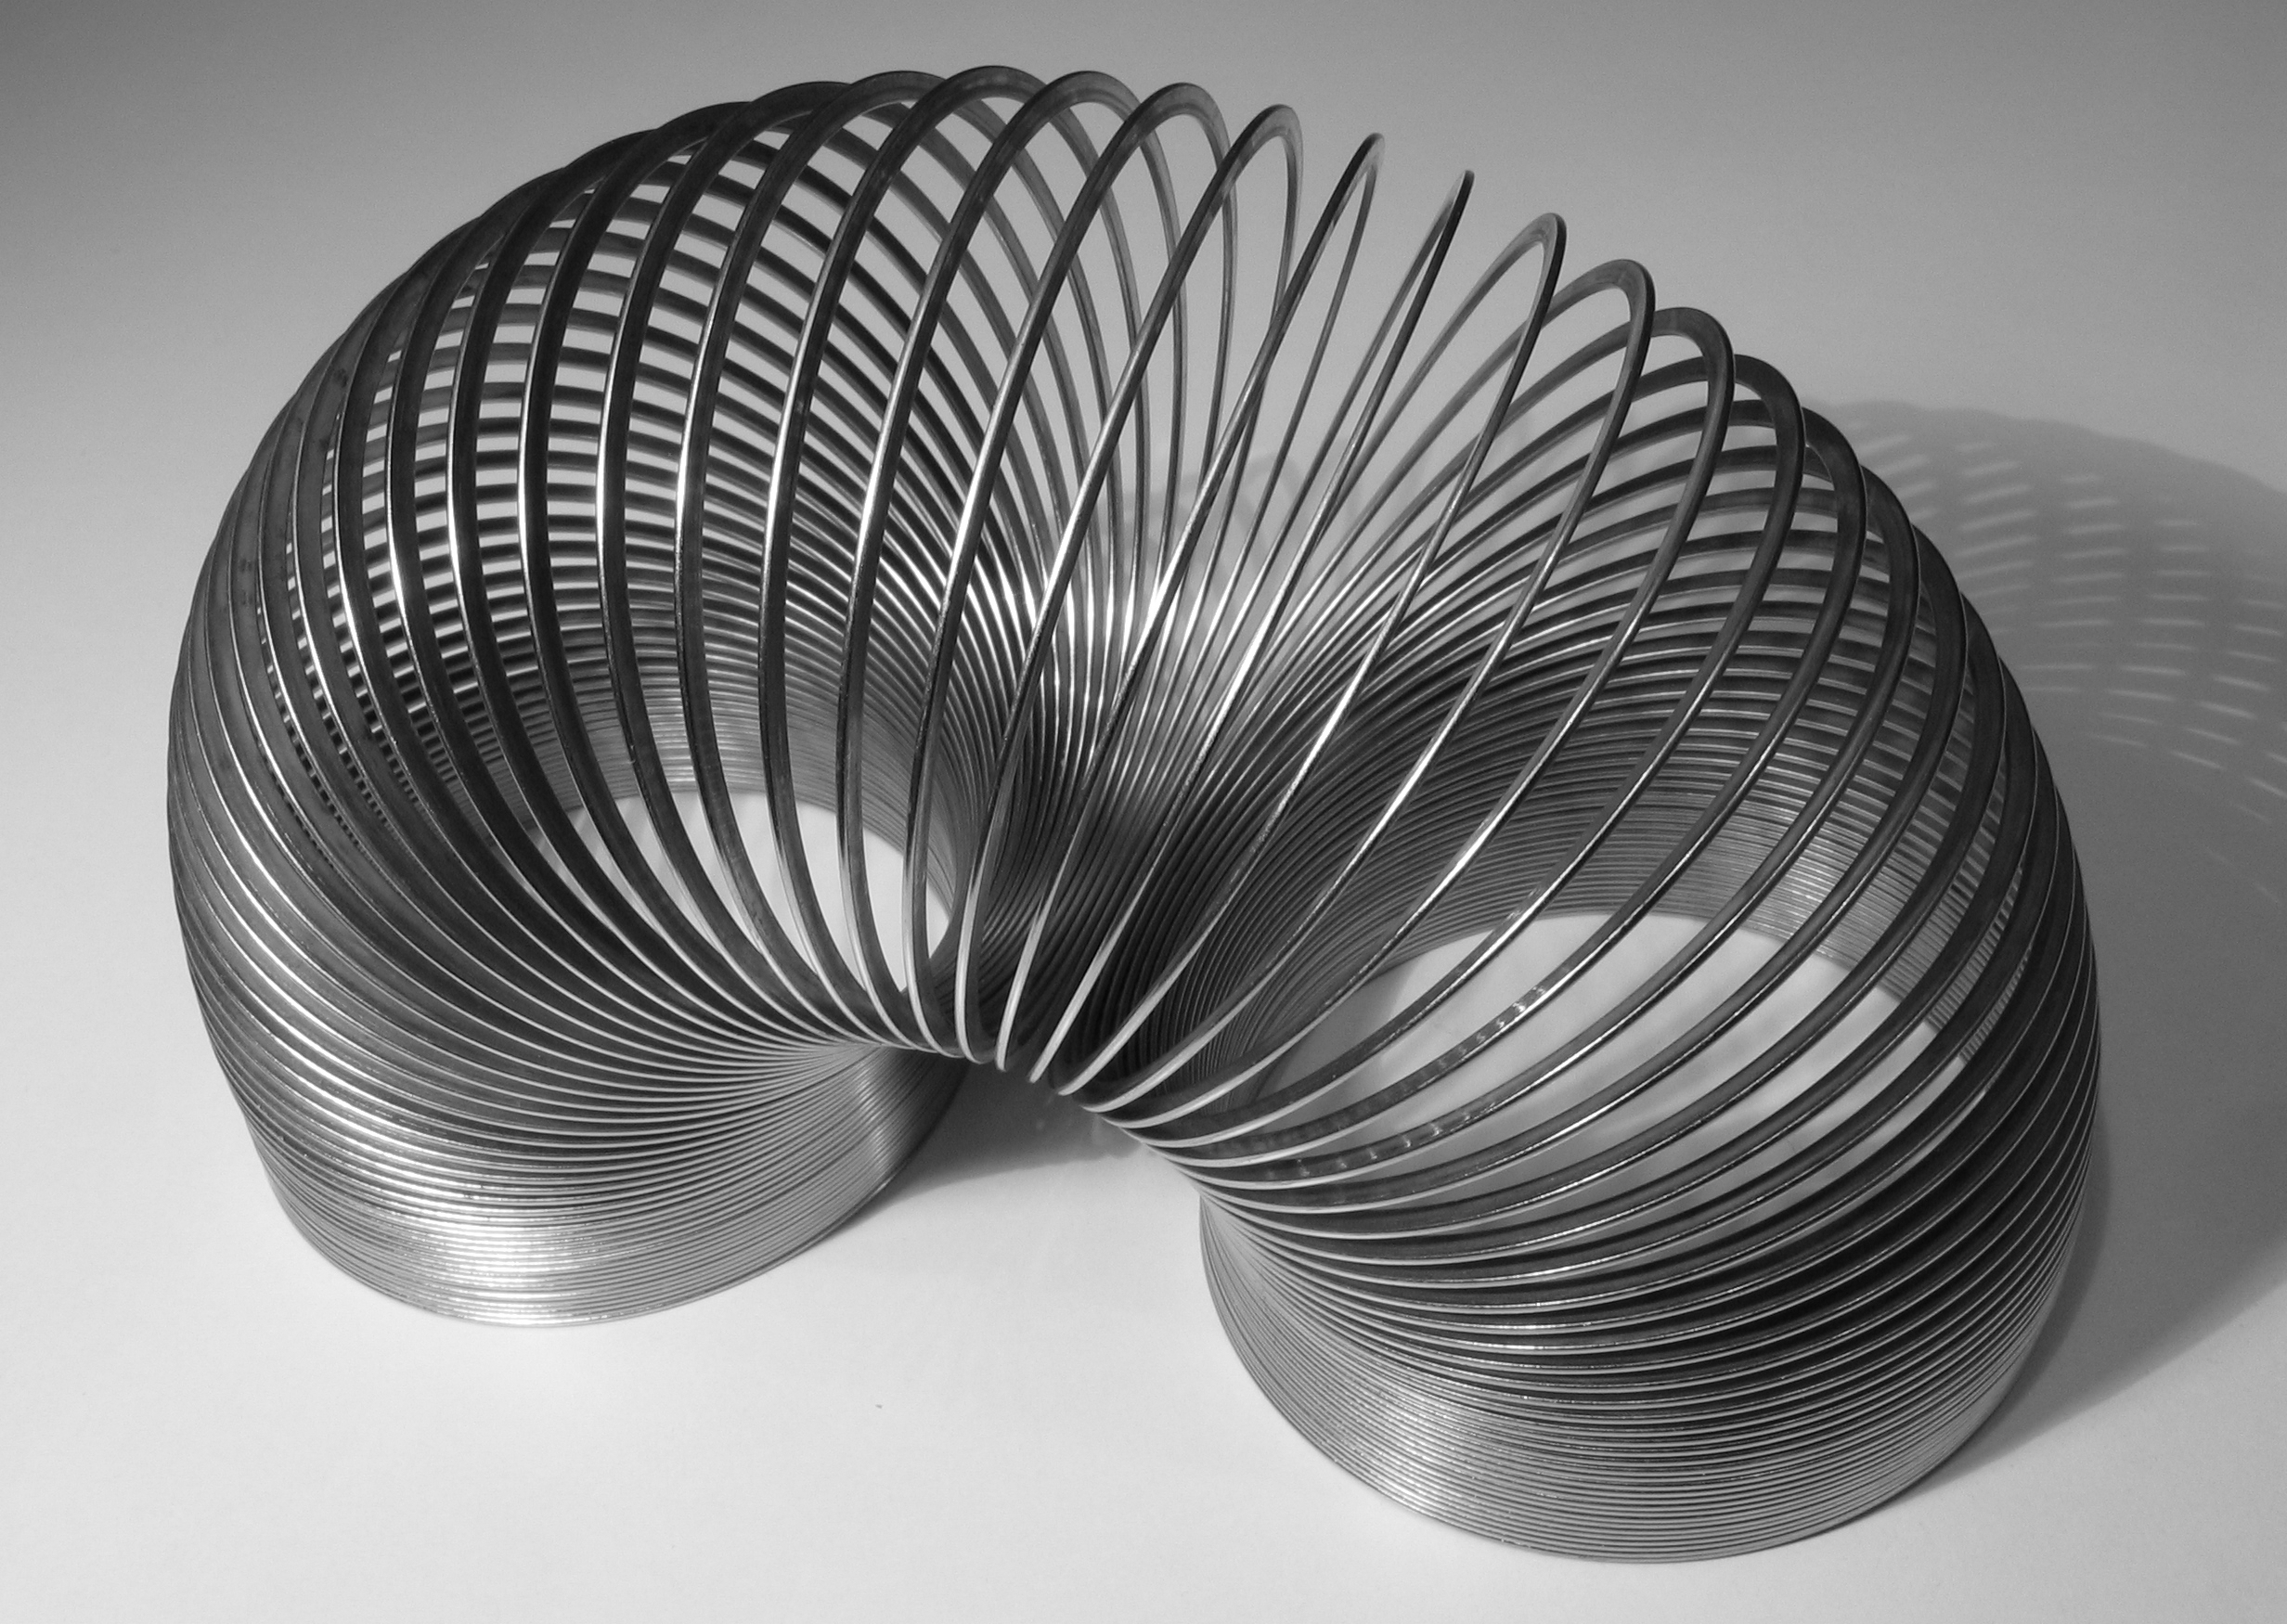
\includegraphics[width=0.45\textwidth]{slinky.jpg}
\quad
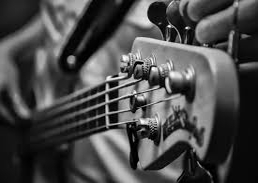
\includegraphics[width=0.45\textwidth]{guitar.jpg}
\end{center}

\section{Linear operators, revisited}

\index{linear operator}

Okay, so what does all this have to do with linear algebra?
